
The \gls{EPICS} and related toolkits can be used to control large experiments or even beamlines, but also smaller experimental setups, in which only limited functionalities are needed. During the R\&D phase for the \gls{STS} many different setups were constructed, in order to evaluate the hardware that should be used for the final experiment. Moreover, challenging ambient conditions of the STS put even more stringent constraints. To address the needs of this dynamic environment, a container-based control framework was implemented. 

Containerization is an increasingly popular method of virtualizing an application, without having to run a full-blown operating system. In modern computing, containers are commonly used both in development and production environments, often together with cloud solutions. In the \gls{HEP} containers and their different applications become more and more popular. According to to~\cite{Klaus2021} the first mention of about a docker container of the \gls{EPICS} \gls{IOC} was related to the Taurus project in 2015~\cite{taurus}. Since then containerization efforts intensified also within the \gls{FAIR} based collaborations - \gls{CBM}/\gls{MVD}~\cite{Klaus2021} and PANDA DCS~\cite{PANDA_1}.

In this chapter, an introduction to the modern control system frameworks is given, together with a detailed explanation of the functionalities of the specific software components. The two following sections introduce the applications of the developed software package for effective control and data acquisition in two chosen setups. The first of mentioned sections focus on the powering irradiation studies and implications for the STS. The last section discusses the results from the thermal cycling activities for the STS electronics, which aimed to discover their operational limitations.
  
\section{Containerized IOC}
IOC container has been prepared by the \gls{DCS} group of the \gls{PANDA} Collaboration and adjusted to the STS needs. The latest IOC's image is built on EPICS R7.0.3.1 image and it contains the most important modules and extensions i.a. asyn, autosave, calc, Modbus, and SNMP (see Figure~\ref{fig_ioc1}). Moreover, by using so-called Volumes (see Figure~\ref{fig_doc}) the \gls{IOC} can be used at any node with the docker engine. Volumes are one of the mechanisms to manage application data and it's a proper way to ensure data persistence. Having prepared database files, st.cmd, and stream protocols if needed, an IOC can be deployed on any node, with any operating system and processor architecture.
\begin{figure}[!h]
\centering
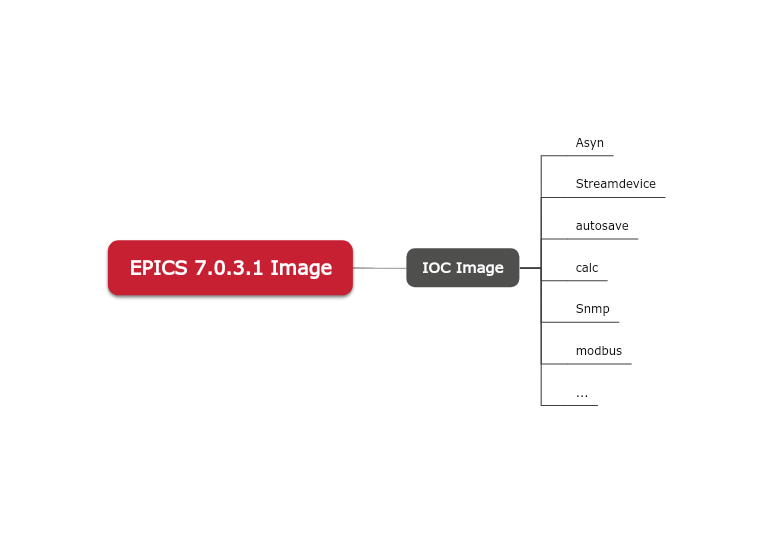
\includegraphics[width=0.65\columnwidth]{Chapter4/images/epics_ioc.png}
\caption{EPICS 7.0.3.1 based IOC image}
\label{fig_ioc1}
\end{figure}
\newpage
A general idea of a containerized \gls{EPICS} \gls{IOC} is presented in the Figure~\ref{fig_doc}. Every container is assigned an IP address for every Docker network it connects to. Moreover, each network has a default subnet mask and gateway. In order to connect the IOC with other services, the ports used by \gls{EPICS} (5064, 5065 for channel access protocol and 7064, 7065 for PVAccess) need to be exposed.  The containers use the host network to communicate with each other and other nodes. It's mostly due to limitations in the protocols used by the \gls{IOC}, as they may not pass through Network Address Translation (NAT).
\begin{figure}[!h]
\centering
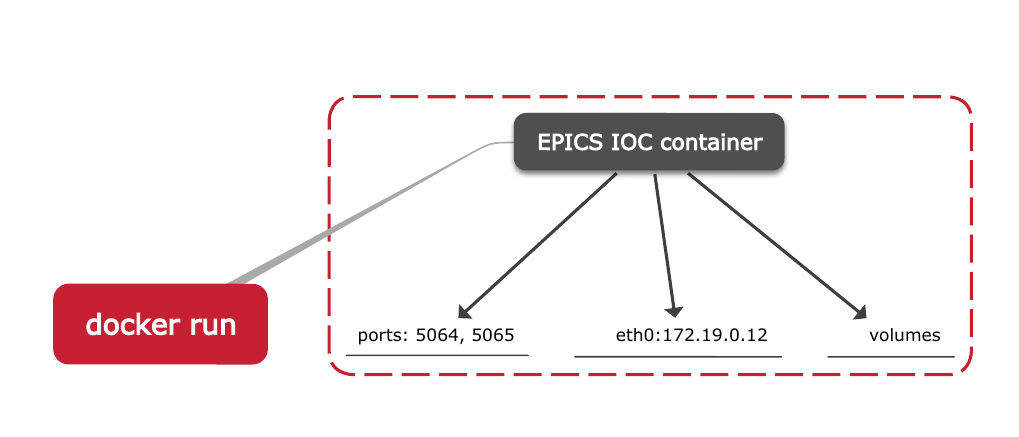
\includegraphics[width=0.7\columnwidth]{Chapter4/images/docker_run.png}
\caption{General idea of an IOC in the container}
\label{fig_doc}
\end{figure}
\newpage
\section{Docker}
Docker was chosen as the platform to prepare the images and run the containers. One of the features of docker has been considered risky for the operation of the detector/experiment, especially considering the final system. Docker-based containers run with the root privileges, therefore posing a threat to the operation of the control system. The daemon is a part of the engine that runs the containers that have full privileges not only within the container but also on the node. If a container gets compromised it may lead to potentially disastrous scenarios, including loss of data or potential threat to the detector - e.g. killing the container. Moreover, a compromised node can also endanger other nodes in the network.  Nevertheless, since late 2020 it's possible to run Docker daemon and containers as a non-root user. Docker daemon and containers themselves can run inside a user namespace~\cite{docker_limitations}, therefore mitigating risk
%\begin{figure}[!h]
%\centering
%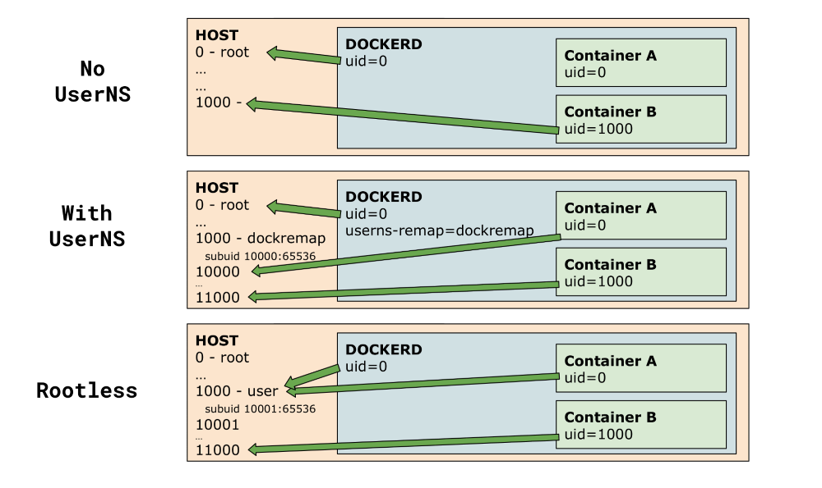
\includegraphics[width=0.8\columnwidth]{sections/images/docker.png}
%\caption{Rootless operation of the container}
%\label{fig_rootless}
%\end{figure}
 Thanks to the Open Container Initiative that defines container formats and runtimes, using different engines doesn't require many changes in the container image. There are also several alternatives to the docker engine, that allow running containers in rootless mode:
\begin{itemize}
    \item Podman~\cite{Podman} 
    \item Singularity~\cite{singularity}
\end{itemize}
\section{Safety Considerations}
Containers are a handy tool to easily address the control and monitoring of different setups. Nevertheless, implementing an additional layer over EPICS-based applications may lead to safety concerns. This technology has many advantages:
\begin{itemize}
    \item standardized, what makes it portable anywhere,
    \item independent of the operating system,
    \item instant replication and easy debugging,
    \item lightweight - containers share the machine's kernel, and they do not require a separate one, which makes them much faster than virtual machines,
    \item docker daemon monitors the containers instead of the hypervisor in case of virtual machines,
    \item processes run as native causing little overhead.
\end{itemize}
For the use of containers in the final experiment, the following list must be taken into consideration:

\begin{itemize}
    \item services should be accessible only by experts, crucial services should be hidden from operators (authorization),
    \item ssh accesses to the DCS nodes should be limited by authorization plugins to avoid overloading,
    \item experiment network should be segmented based on the goals and communication between software entities clearly, defined (\gls{DCS}, \gls{SCA})
    \item proper security context for all the services (e.g. root privileges),
    \item logging all the changes in the cluster,
    \item preventing containers from loading unwanted kernel modules,
    \item cluster and container redundancy.
\end{itemize}

\section{Motivation}
Nevertheless, to demonstrate the containerized \gls{DCS}, not all the available applications were used. The mSTS's \gls{DCS} features the applications listed in the figure \ref{fig_dcs_node_msts}. All these applications were used as containers based on previously prepared images and linked using Docker-compose, which is a tool for defining and running multi-container Docker applications \cite{docker_compose}. To configure the containers a YAML file has to be populated with the container settings. This section summarizes the most important applications used for the DCS and their functionalities.
